% ======================================================================
\chapter{Search Strings and Sources}
\label{app:search}
% ======================================================================

All searches were run on 31 October 2026 for publication years 2016--2026. The raw responses are stored in \texttt{review/data/raw/}.

\paragraph{OpenAlex (executed).} Works endpoint, Boolean search over titles and abstracts, page paging, 200 records per page:
\begin{small}
\begin{verbatim}
filter = title_and_abstract.search:("reinforcement learning" OR
         "imitation learning") AND ("congestion control" OR
         "congestion window" OR ECN),publication_year:2016-2026
\end{verbatim}
\end{small}

\paragraph{arXiv (executed).} Because the API's phrase operator under-retrieves, we retrieved on single terms and applied the protocol's exact phrases locally (hyphens treated as spaces; ``ECN'' matched as a whole word):
\begin{small}
\begin{verbatim}
search_query = (ti:reinforcement OR abs:reinforcement OR ti:imitation
                OR abs:imitation) AND (ti:congestion OR abs:congestion
                OR ti:ECN OR abs:ECN)
                AND submittedDate:[201601010000 TO 202612312359]
\end{verbatim}
\end{small}

\paragraph{USENIX NSDI and ATC (executed).} The technical-sessions page of every NSDI (2016--2026) and USENIX ATC (2016--2025) was scraped for titles and abstracts, and the protocol query was applied locally.

\paragraph{Subscription databases (for re-execution with institutional access).} These strings implement the same query in each database's syntax. We could not run them (\cref{sec:search}).
\begin{small}
\begin{verbatim}
IEEE Xplore (Command Search; Publication Year 2016-2026):
  (("Document Title":"reinforcement learning" OR
    "Abstract":"reinforcement learning" OR
    "Document Title":"imitation learning" OR
    "Abstract":"imitation learning") AND
   ("Document Title":"congestion control" OR
    "Abstract":"congestion control" OR
    "Document Title":"congestion window" OR
    "Abstract":"congestion window" OR
    "Document Title":ECN OR "Abstract":ECN))

ACM Digital Library (Advanced Search; Published 2016-2026):
  (Title:("reinforcement learning" OR "imitation learning") OR
   Abstract:("reinforcement learning" OR "imitation learning")) AND
  (Title:("congestion control" OR "congestion window" OR ECN) OR
   Abstract:("congestion control" OR "congestion window" OR ECN))

Scopus (Advanced Search):
  TITLE-ABS(("reinforcement learning" OR "imitation learning") AND
            ("congestion control" OR "congestion window" OR ecn))
  AND PUBYEAR > 2015 AND PUBYEAR < 2027
\end{verbatim}
\end{small}

\paragraph{Citation searching.} \emph{Forward}: all 2016--2026 works citing at least one of ten seed reports and mentioning ``congestion'' in the title or abstract. The seeds were Aurora (arXiv 2018 and ICML 2019), Orca, Pantheon/Indigo, MVFST-RL, Sage, QTCP, Eagle, TCP-RL, and DRL-CC for MPTCP. \emph{Backward}: the reference lists of sixteen recent included reports with long related-work sections. Sage, Orca and Astraea were among them, and the full list is stored with the raw responses. Records already identified were removed before screening.

\paragraph{Supplementary search for LLM-based work (\cref{sec:llm}).} This scoped search informs the narrative of \cref{sec:llm} only and did not enter the PRISMA flow:
\begin{small}
\begin{verbatim}
OpenAlex (2022-2026, titles and abstracts):
  ("large language model" OR "large language models" OR LLM OR LLMs
   OR "language model" OR GPT) AND
  ("congestion control" OR "congestion window")
arXiv (2022-2026), then a local filter for "congestion control|window":
  (ti:LLM OR abs:LLM OR ti:LLMs OR abs:LLMs OR ti:"language model"
   OR abs:"language model" OR abs:"language models") AND
  (ti:congestion OR abs:congestion)
\end{verbatim}
\end{small}

% ======================================================================
\chapter{Additional Tables and Figures}
\label{app:tables}
% ======================================================================

\begin{small}
\setlength{\tabcolsep}{4pt}
\begin{longtable}{@{}L{4.0cm}lL{8.6cm}@{}}
\caption{The \nLevelRealnetwork{} studies whose evaluation reaches a real network, and what that network was. Production deployments and A/B tests are rare; most ``real'' evaluations use cloud or testbed hosts on Internet paths.}\label{tab:real}\\
\toprule Study & Year & Real-network evaluation \\ \midrule \endfirsthead
\toprule Study & Year & Real-network evaluation \\ \midrule \endhead
\bottomrule \endfoot
Pantheon (Indigo)~\cite{yan2018pantheon} & 2018 & Pantheon nodes on real Internet paths (wired and cellular, several countries) \\
TCP-RL~\cite{nie2019tcprl} & 2018 & production web servers of a top global search engine (>1 year) \\
Concerto~\cite{zhou2019concerto} & 2019 & operational mobile video-telephony service \\
DRL-CCP~\cite{lan2019deep} & 2019 & physical NDN test platform \\
RL BWE for RTC (Microsoft)~\cite{fang2019rtc} & 2019 & real Internet video calls \\
ARC~\cite{zhang2020reinforcement} & 2020 & real testbed (training and test) \\
DeepCC (Abbasloo et al.)~\cite{abbasloo2021deepcc} & 2020 & real-world cellular experiments \\
OnRL~\cite{zhang2020onrl} & 2020 & Alibaba Taobao-live (543 h, 151 users) \\
Orca~\cite{abbasloo2020orca} & 2020 & global Internet testbeds (cloud servers across continents) \\
ACC~\cite{yan2021acc} & 2021 & production DCs (300 machines, storage service) \\
AUTO~\cite{li2021auto} & 2021 & real Internet paths (cloud) \\
Libra~\cite{du2025libra} & 2021 & live Internet paths \\
Loki~\cite{zhang2021loki} & 2021 & commercial real-time video system (101M sessions) \\
MOCC~\cite{ma2022mocc} & 2021 & real-world Internet experiments \\
RLCC~\cite{xia2021rlcc} & 2021 & Pantheon nodes on AWS \\
BBR-FIT~\cite{xie2022bbr} & 2022 & real 5G/WiFi testbed \\
DeepCC (Zhang et al.)~\cite{zhang2022deepcc} & 2022 & inter-continental real-world paths \\
DuGu~\cite{huang2022learned} & 2022 & real-world A/B tests in a short-video upload service \\
Genet~\cite{xia2022genet} & 2022 & real-world network paths \\
HybridRTS~\cite{zhang2022hybridrts} & 2022 & real-world WebRTC experiments \\
MP-OL~\cite{zhuang2022achieving} & 2022 & real networks \\
OpenNetLab~\cite{eo2022opennetlab} & 2022 & distributed real-network testbed nodes \\
RL-CC on NVIDIA NICs~\cite{fuhrer2023nvidia} & 2022 & live cluster with NVIDIA ConnectX NICs \\
Spine~\cite{tian2024spine} & 2022 & real-world Internet experiments \\
ZiXia~\cite{jia2022zixia} & 2022 & global real-world paths \\
Dolce-RC~\cite{ye2023data} & 2023 & commodity SmartNIC testbed \\
Floo~\cite{zhang2023floo} & 2023 & production mobile web service \\
Leopard~\cite{liu2023leopard} & 2023 & real-world experiments \\
MARLIN~\cite{galliera2023marlin} & 2023 & real network with background traffic (training and test) \\
MIQA / MIA~\cite{wu2024miqa} & 2023 & mmWave immersive testbed \\
Marten~\cite{zhou2025safety} & 2023 & production network (QUIC) \\
Sage~\cite{yen2023sage} & 2023 & Internet paths \\
Astraea~\cite{liao2024astraea} & 2024 & inter-continental real-world paths (cloud) \\
Canopy~\cite{yang2024canopy} & 2024 & global testbed \\
MMSys'24 offline-RL BWE challenge~\cite{khairy2024acm} & 2024 & real-world RTC evaluation \\
Maggey~\cite{wei2024breaking} & 2024 & live experiments \\
SAC-MWL (QUIC)~\cite{blokhin2024deep} & 2024 & worldwide real network endpoints \\
Anole~\cite{han2025anole} & 2025 & real-world wired and Wi-Fi networks \\
D2T*~\cite{liu2025automatic} & 2025 & P4-programmable switch \\
EchoCC~\cite{yu2025echocc} & 2025 & live Internet \\
Flecto~\cite{serra2025flecto} & 2025 & 5G testbed (OpenAirInterface + USRP B210) \\
GO RL TL (semantic CC)~\cite{kutsevol2025learning} & 2025 & hardware tests \\
Jazz~\cite{wang2025edge} & 2025 & dual-band (5/6 GHz) Wi-Fi testbed \\
Jury~\cite{tian2025jury} & 2025 & real-world Internet paths \\
Mona adversarial policy~\cite{chen2025exploring} & 2025 & real-world network deployments \\
Mutant~\cite{pappone2025mutant} & 2025 & inter-continental real-world paths \\
ICCP~\cite{ji2026iccp} & 2026 & real-world experiments \\
PPO CC on a 10 Gb/s WAN~\cite{ghermezian2026ppo} & 2026 & real 10 Gbit/s high-BDP WAN path \\
TCCO~\cite{zhang2026transformer} & 2026 & dual-band Wi-Fi testbed \\
\end{longtable}
\end{small}


\begin{figure}[ht]
\centering
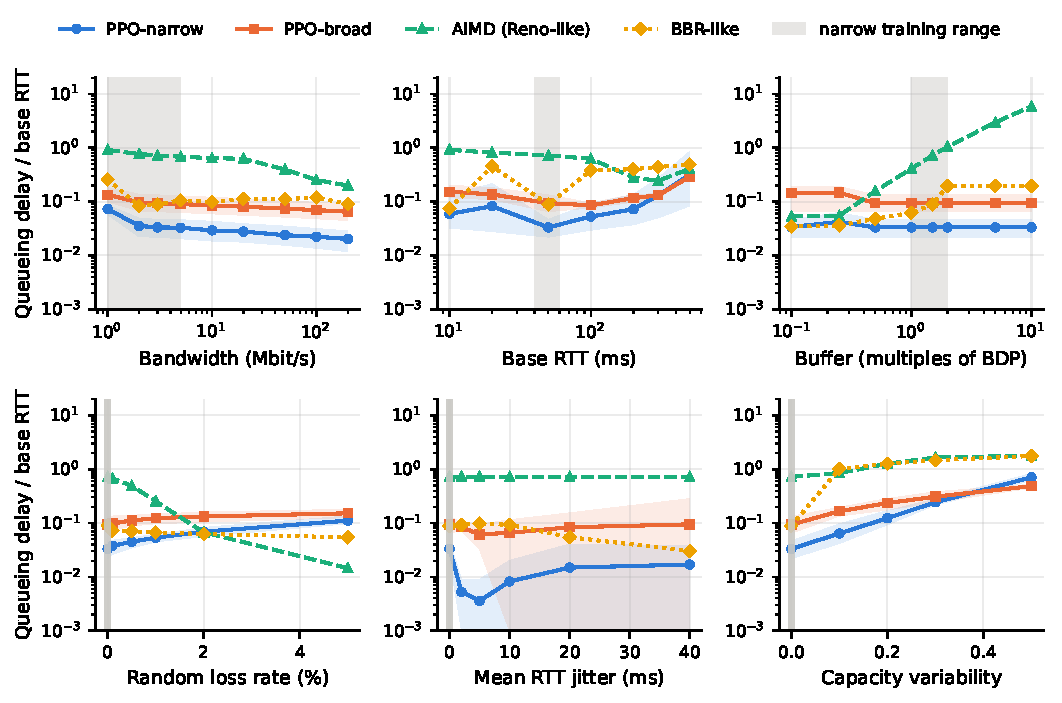
\includegraphics[width=\linewidth]{figures/case_study_delay.pdf}
\caption{Case study: mean queueing delay (in multiples of the base RTT, log scale) when one factor is varied around the reference link. Lines are means over the converged training seeds (as in \cref{tab:case}) and shaded bands span them; the gray band or line marks the narrow training range. Both PPO policies keep queues far shorter than AIMD and usually shorter than BBR-like. Under capacity variability all controllers queue more, the classic ones most.}
\label{fig:case-delay}
\end{figure}

\clearpage
\begin{small}
\setlength{\tabcolsep}{3pt}
\begin{longtable}{@{}L{4.2cm}lllL{4.6cm}ll@{}}
\caption{All \nStudies{} included studies, ordered by year of first report. Setting: WAN = Internet/wide-area, Gen.\ = unspecified/generic, Wless = wireless/cellular, Sat.\ = satellite/space, IoT = IoT/ad hoc/sensor, DC = data center. Level: highest evaluation environment reported (Sim/Emu/Real; NR = not reported; -- = formal analysis only). Code: \cmark{} = artifact released. Linked reports of the same study are cited together.}\label{tab:all-studies}\\
\toprule Study & Year & Set. & Action & Method & Level & Code \\ \midrule \endfirsthead
\toprule Study & Year & Set. & Action & Method & Level & Code \\ \midrule \endhead
\bottomrule \endfoot
Q-learning TCP for memory-constrained IoT~\cite{li2016learning} & 2016 & IoT & cwnd & Q-learning with function approximation & Sim &  \\
Smart-DTN-CC~\cite{silva2019congestion,silva2016smart} & 2016 & IoT & other & RL & Sim &  \\
Kanerva-coding RL TCP~\cite{li2017dynamic} & 2017 & Gen. & cwnd & Q-learning + generalization-based Kanerva cod… & NR &  \\
Actor-critic AQM~\cite{xu2018network} & 2018 & Gen. & AQM & actor-critic & Sim &  \\
Aurora~\cite{jay2019aurora,jay2018internet} & 2018 & WAN & rate & PPO & Emu & \cmark \\
Iroko~\cite{ruffy2018iroko} & 2018 & DC & rate & PPO; REINFORCE; DDPG & Emu & \cmark \\
Muses~\cite{zhong2022muses,wang2018muses} & 2018 & Wless & cwnd & imitation-learned LSTM distilled into per-env… & NR &  \\
Pantheon (Indigo)~\cite{yan2018pantheon} & 2018 & WAN & cwnd & imitation learning from emulator oracles & Real & \cmark \\
QARC~\cite{huang2018qarc} & 2018 & WAN & bitrate & A3C + video-quality prediction network & Sim &  \\
QTCP~\cite{li2019qtcp} & 2018 & Gen. & cwnd & Q-learning + generalized Kanerva coding & NR &  \\
RL-TCP~\cite{kong2018improving} & 2018 & Gen. & cwnd & Q-learning & Sim &  \\
SDN-DC Q-learning/SARSA CC~\cite{jin2018congestion} & 2018 & DC & rate & Q-learning; SARSA & NR &  \\
TCP-RL~\cite{nie2019tcprl,nie2018smartiw} & 2018 & WAN & param., select & group-based RL + deep RL & Real &  \\
eqCC~\cite{trinh2018energy} & 2018 & IoT & rate & Q-learning & Sim &  \\
Concerto~\cite{zhou2019concerto} & 2019 & WAN & bitrate & custom imitation learning on >1M logged sessi… & Real &  \\
DRL fronthaul CC~\cite{nascimento2019deep} & 2019 & Wless & rate & several DRL methods & Sim &  \\
DRL initial window for 5G MEC~\cite{xie2019adaptive} & 2019 & Wless & param. & DRL & Sim &  \\
DRL-CC (MPTCP)~\cite{xu2019drlcc} & 2019 & Gen. & cwnd & deterministic policy gradient actor-critic +… & Emu &  \\
DRL-CCP~\cite{lan2019deep} & 2019 & WAN & rate & DRL & Real &  \\
Intelligent AQM with ECN~\cite{gomez2019intelligent} & 2019 & Gen. & AQM & Q-learning & Emu &  \\
LGFCC~\cite{wang2019reinforcement} & 2019 & Sat. & other & RL + incomplete-information game & Sim &  \\
MVFST-RL~\cite{sivakumar2019mvfst} & 2019 & WAN & cwnd & IMPALA with delayed actions & Emu & \cmark \\
RL BWE for RTC (Microsoft)~\cite{fang2019rtc} & 2019 & WAN & bitrate & PPO & Real &  \\
RL loss-differentiating TCP~\cite{rani2019reinforcement} & 2019 & Wless & cwnd & RL & NR &  \\
Rax~\cite{bachl2019rax} & 2019 & Gen. & cwnd & online deep RL with Partial Action Learning & NR &  \\
Robustifying protocols with adversarial examples~\cite{gilad2019robustifying} & 2019 & Gen. & -- & RL-generated adversarial network conditions & Sim &  \\
SmartCC~\cite{li2019smartcc} & 2019 & Wless & cwnd & Q-learning + hierarchical tile coding & NR &  \\
TCP-Drinc~\cite{xiao2019drinc} & 2019 & Gen. & cwnd & DQN with CNN+LSTM & Sim &  \\
Verily~\cite{kazak2019verily} & 2019 & Gen. & -- & formal verification of DRL policies & -- &  \\
ARC~\cite{zhang2020reinforcement} & 2020 & WAN & cwnd & asynchronous RL trained in real networks & Real &  \\
DeepCC (Abbasloo et al.)~\cite{abbasloo2021deepcc} & 2020 & Wless & param. & DDPG plug-in capping the cwnd of existing TCP & Real & \cmark \\
Distributed RL in-network CC~\cite{mai2020distributed} & 2020 & Gen. & rate & CTDE with centralized critic & Sim &  \\
Eagle~\cite{emara2020eagle} & 2020 & WAN & rate & DRL with LSTM guided by BBR as expert & Emu &  \\
Hd-TCP~\cite{cui2020improving} & 2020 & Wless & cwnd & DRL & Sim &  \\
LFQ~\cite{bachl2020lfq} & 2020 & Gen. & buffer & online DRL & Sim & \cmark \\
Metis~\cite{meng2020interpreting} & 2020 & Gen. & -- & decision-tree and hypergraph interpretation o… & Sim & \cmark \\
Multi-task DRL CC (SDN)~\cite{lei2020congestion} & 2020 & Gen. & rate & multi-task DRL & NR &  \\
OnRL~\cite{zhang2020onrl} & 2020 & Wless & bitrate & online RL: per-user agents, aggregated model… & Real &  \\
Orca~\cite{abbasloo2020orca} & 2020 & WAN & cwnd & TD3 & Real & \cmark \\
Partner~\cite{huang2020objective} & 2020 & Gen. & cwnd & distributed DRL & NR &  \\
RLAQM~\cite{jiang2020performance} & 2020 & Gen. & AQM & Q-learning & Sim &  \\
RTCP (HSR)~\cite{xu2020handover} & 2020 & Wless & cwnd & DRL & Sim &  \\
SDN actor-critic MPTCP for IoT~\cite{naeem2020software} & 2020 & IoT & cwnd & actor-critic with fuzzy normalized NN & Sim &  \\
TCP-PPCC~\cite{li2020tcp} & 2020 & Gen. & cwnd & PPO & Sim &  \\
ACC~\cite{yan2021acc} & 2021 & DC & ECN thr. & multi-agent DRL per switch & Real &  \\
AIMD-QTCP~\cite{yamazaki2021fairness} & 2021 & Gen. & cwnd & Q-learning + AIMD window rule & Sim &  \\
AQM meets DRL~\cite{ma2021intelligent} & 2021 & Gen. & AQM & DRL & NR &  \\
AUTO~\cite{li2021auto} & 2021 & Sat. & rate & multi-objective RL + preference-adaptation mo… & Real &  \\
Arsenal~\cite{zhang2021arsenal} & 2021 & Wless & -- & evaluation platform for AI-driven video trans… & Sim &  \\
CRL-CC~\cite{liu2021multi} & 2021 & WAN & rate & constrained RL & Emu &  \\
DQL-MPTCP~\cite{pokhrel2021learning} & 2021 & Gen. & cwnd, split & deep Q-learning with policy gradients, LSTM… & Emu &  \\
DRL-3R~\cite{chen2021ran,chen2021rana} & 2021 & Wless & cwnd & DRL with reward redistribution & NR &  \\
DRL-CC (deadline-aware)~\cite{liao2021learning} & 2021 & Gen. & rate & DRL & NR &  \\
DeepCC (He et al., MPTCP)~\cite{he2021deepcc} & 2021 & Wless & cwnd & multi-agent DRL with self-attention & NR &  \\
HRCC~\cite{wang2021hybrid} & 2021 & WAN & param. & RL agent sets a gain on the heuristic bandwid… & Sim &  \\
HSR-CC (space-ground MPTCP)~\cite{xu2021deep} & 2021 & Sat. & cwnd & DRL & NR &  \\
LearningCC~\cite{zhang2021learningcc} & 2021 & Gen. & cwnd & multi-armed bandit over cwnd update rules & Sim &  \\
Libra~\cite{du2025libra,du2021libra} & 2021 & WAN & rate & classic and RL candidates compared in explora… & Real &  \\
Loki~\cite{zhang2021loki} & 2021 & WAN & bitrate & RL model fused with a reverse-engineered rule… & Real &  \\
MARL + transfer TCP CC~\cite{kasi2021tcp} & 2021 & Gen. & cwnd & transfer-learning-assisted RL; coordinated MA… & NR &  \\
MOCC~\cite{ma2022mocc,ma2021multi} & 2021 & WAN & rate & PPO with preference sub-network + transfer le… & Real &  \\
MOCC (Xia et al.)~\cite{xia2021multi} & 2021 & WAN & rate & multi-objective RL with preferences & NR &  \\
MPLibra~\cite{yu2024classic,yu2021mplibra} & 2021 & Gen. & select & classic and learned MPTCP decisions compared… & Sim &  \\
Owl~\cite{sacco2021owl,sacco2022partially} & 2021 & WAN & cwnd & DQN in a Linux kernel module & Emu &  \\
Policy distillation (fronthaul)~\cite{martins2021policy} & 2021 & Wless & rate & TD3 distilled into decision trees / C++ rules & Sim & \cmark \\
RL-PSD~\cite{xu2021reinforcement} & 2021 & Wless & cwnd & two-stage RL & NR &  \\
RL-explore~\cite{li2021tcp} & 2021 & Gen. & cwnd & RL + bandwidth-probing mechanism & NR &  \\
RLCC~\cite{xia2021rlcc} & 2021 & WAN & cwnd & DQN & Real &  \\
Rainbow vs DQN for TCP CC~\cite{martins2021rainbow} & 2021 & Gen. & cwnd & Rainbow and DQN extensions & Sim &  \\
SDN Q-learning rate allocation~\cite{zhang2021research} & 2021 & Gen. & rate & Q-learning & Emu &  \\
TCP-DQN~\cite{wang2021intelligent} & 2021 & WAN & cwnd & DQN & NR &  \\
TCP-NeuRoc~\cite{li2021tcpa} & 2021 & Gen. & cwnd & DRL + online changepoint detection; cold-star… & Emu &  \\
TCP-RL in an SDN data centre~\cite{hassan2021tcp} & 2021 & DC & cwnd & RL & NR &  \\
TD actor-critic TCP~\cite{pradeep2021temporal} & 2021 & Wless & cwnd & actor-critic TD learning & NR &  \\
Teacher-Student robust DRL~\cite{zheng2022teacher,zheng2021leveraging} & 2021 & Gen. & rate & teacher advice + reward shaping + prioritized… & Sim &  \\
Zwei~\cite{huang2021zwei} & 2021 & WAN & bitrate & self-play RL using the actual requirement as… & Sim &  \\
whiRL 2.0~\cite{eliyahu2021whirl} & 2021 & Gen. & -- & DNN verification + model checking of DRL poli… & -- &  \\
Adversarial attack on RL CC~\cite{yang2022good} & 2022 & Gen. & -- & state-estimating adversarial perturbation att… & Sim &  \\
BBR-FIT~\cite{xie2022bbr} & 2022 & Wless & param. & RL tunes BBR gain & Real &  \\
BoB~\cite{bentaleb2022bob} & 2022 & WAN & bitrate & PPO + heuristic warm start & Emu & \cmark \\
CLCC~\cite{li2022reinforcement} & 2022 & WAN & bitrate & RL with frame-level features & Sim &  \\
Coefficient-free RL rate control~\cite{xiao2022optimal} & 2022 & DC & rate & RL with coefficient-free objective & NR &  \\
DQN TCP v2 fairness~\cite{seo2022fairness} & 2022 & Gen. & cwnd & DQN & Sim &  \\
DQN-tuned AQM~\cite{yousif2022intelligent} & 2022 & Gen. & AQM & DQN & Sim &  \\
DRL bidirectional-node WSN CC~\cite{lei2022deep} & 2022 & IoT & rate & DRL & Sim &  \\
DRL-CC ablation (cellular)~\cite{naqvi2022ablation} & 2022 & Wless & rate & ablation of DRL training choices & Sim &  \\
DeepCC (Zhang et al.)~\cite{zhang2022deepcc} & 2022 & WAN & rate & DDPG-based multi-objective offline training +… & Real &  \\
DuGu~\cite{huang2022learned} & 2022 & WAN & rate & NN imitates an optimal solver in an omniscien… & Real &  \\
Federated DRL bandwidth weights~\cite{liu2022distributed} & 2022 & WAN & param. & federated multi-agent DRL & NR &  \\
GDMD~\cite{yang2022gdmd} & 2022 & Gen. & rate & RL CC + block scheduler & NR &  \\
Genet~\cite{xia2022genet,xia2022automatic} & 2022 & WAN & rate & curriculum learning promoting environments wh… & Real & \cmark \\
Glider~\cite{xia2022glider} & 2022 & WAN & rate & DRL & Emu &  \\
HybridRTS~\cite{zhang2022hybridrts} & 2022 & WAN & bitrate & switching between rule-based and RL rate cont… & Real &  \\
ICCDRL~\cite{wang2022intelligent} & 2022 & Wless & cwnd & DRL & Sim &  \\
IEACC~\cite{yang2022ieacc} & 2022 & WAN & rate & DRL with edge-aided congestion degrees & Sim &  \\
LiteFlow~\cite{zhang2022liteflow,zhang2023liteflow} & 2022 & Gen. & rate & kernel fast path for NN inference + userspace… & Emu &  \\
MACC (cross-layer)~\cite{bai2022macc,bai2023ma} & 2022 & Gen. & cwnd, AQM & two cooperating DQN agents & Sim &  \\
MP-OL~\cite{zhuang2022achieving} & 2022 & Gen. & rate & multi-armed bandit per subflow, switchable to… & Real &  \\
NCC~\cite{wang2022ncc} & 2022 & DC & rate & RL & Emu &  \\
Nuwa-RL~\cite{gong2022nuwa,jiang2025combining} & 2022 & Wless & param. & PPO-LSTM tunes receiver-side heuristic & NR &  \\
OAC-TCPCC~\cite{masood2022intelligent} & 2022 & Sat. & cwnd & optimistic actor-critic & Sim &  \\
OpenNetLab~\cite{eo2022opennetlab} & 2022 & WAN & bitrate & platform for training/evaluating RL RTC CC & Real & \cmark \\
Pareto~\cite{emara2022pareto} & 2022 & WAN & rate & communication-free MARL, staged training + on… & NR &  \\
Plume (lightweight DRL CC)~\cite{wei2022plume} & 2022 & Gen. & rate & compressed DRL framework; reward re-parameter… & NR &  \\
Q-learning adaptive TCP CC~\cite{satinge2022q} & 2022 & Gen. & cwnd & Q-learning & NR &  \\
RL local flow control (lossy networks)~\cite{forero2022congestion} & 2022 & IoT & rate, buffer & RL + portfolio-based buffer allocation & Sim &  \\
RL-CC (Tessler et al.)~\cite{tessler2022rlcc} & 2022 & DC & rate & policy gradient with analytic reward derivati… & Sim &  \\
RL-CC on NVIDIA NICs~\cite{fuhrer2023nvidia} & 2022 & DC & rate & RL-CC policy distilled into decision trees & Real & \cmark \\
RLRBM~\cite{ma2022rlrbm} & 2022 & Wless & buffer & DRL & Sim &  \\
RSCAT~\cite{diel2023rscat,diel2022data} & 2022 & DC & param. & actor-critic RL + congestion classification & NR &  \\
SAC-CC~\cite{guo2022deep} & 2022 & Gen. & rate & SAC with GRU + self-attention & NR &  \\
SDN-DC incast DRL~\cite{guo2022congestion} & 2022 & DC & rate & DRL & Sim &  \\
Scenario-based modelling for DRL (Aurora)~\cite{yerushalmi2023enhancing,yerushalmi2022scenario} & 2022 & WAN & rate & PPO with scenario-based reward shaping & Sim &  \\
Spine~\cite{tian2024spine,tian2022spine} & 2022 & WAN & param. & hierarchical: light CC executor + coarse-grai… & Real &  \\
Symbolic distillation~\cite{sharan2022symbolic} & 2022 & WAN & rate & Aurora PPO policy distilled into symbolic tre… & Emu & \cmark \\
TCP-CFCC~\cite{huang2022tcp} & 2022 & WAN & rate & PPO & Emu &  \\
Transformer-BBR (power IoT)~\cite{li2022noninvasive} & 2022 & IoT & cwnd & DRL with Transformer agent in BBR probing & Sim &  \\
ZiXia~\cite{jia2022zixia} & 2022 & WAN & rate & DRL with adjusted ranking reward & Real &  \\
A2C UAV bottleneck control~\cite{feng2023deep} & 2023 & Wless & rate & A2C & Sim &  \\
ABBR~\cite{pan2023making} & 2023 & WAN & rate & DRL with BBR domain knowledge & Emu &  \\
ACC-RL (power DC)~\cite{huang2023acc} & 2023 & DC & rate & deterministic policy gradient & Sim &  \\
ACCT~\cite{kheirkhah2023acct} & 2023 & Gen. & param. & actor-critic with multiple reward functions & Sim &  \\
ACoCo~\cite{jayaudhaya2023acoco} & 2023 & IoT & param. & RL adapts CoAP CC parameters & Sim &  \\
CARLA~\cite{zhou2023congestion} & 2023 & IoT & rate & learning automata & Sim & \cmark \\
DECC~\cite{liu2023decc} & 2023 & DC & cwnd & DRL + ECN with decoupled cwnd adjustment & Sim &  \\
DLCC~\cite{hou2023deep} & 2023 & IoT & rate & DRL in a non-cooperative Markov game with Lag… & Sim &  \\
DNN+DRL wireless CC~\cite{midhula2023adaptive} & 2023 & Wless & cwnd & DRL & NR &  \\
DRL CC for SDN/NDN satellites~\cite{xing2023deep} & 2023 & Sat. & NR & DRL & NR &  \\
DRLFcc~\cite{cao2023drlfcc} & 2023 & Wless & cwnd & DRL combined with fast recovery & Sim &  \\
DeepFC~\cite{he2023fine} & 2023 & IoT & param., cwnd & DRL predicts transmission-unit size coupled w… & NR &  \\
Distributed RL training system for CC~\cite{luo2023novel} & 2023 & Gen. & -- & distributed sample generation + online analys… & NR &  \\
Dolce-RC~\cite{ye2023data} & 2023 & DC & param. & multi-armed bandit over rate-increase/decreas… & Real &  \\
Floo~\cite{zhang2023floo} & 2023 & WAN & select & RL-based CCA selection with smooth switching & Real &  \\
Hierarchical MARL queue policies (maritime)~\cite{forero2023learning} & 2023 & IoT & rate, other & hierarchical multi-agent RL & Sim &  \\
Implementability of DRL CC (cellular)~\cite{naqvi2023implementability} & 2023 & Wless & NR & DRL & NR &  \\
Internet CC benchmarking~\cite{abbasloo2023internet} & 2023 & WAN & -- & general benchmarks ranking Internet CCs incl… & Emu &  \\
Interval configuration for DRL CC~\cite{naqvi2023fine} & 2023 & WAN & rate & PPO with different MI / RTT estimators & Emu &  \\
Inverse-RL CC~\cite{luo2023novela} & 2023 & Gen. & NR & inverse RL with parallel training & NR &  \\
IoUT CoAP copies~\cite{tariq2023ai} & 2023 & IoT & param. & RL at the sink sets per-node copy count & Sim &  \\
LRCC~\cite{du2023learning} & 2023 & WAN & bitrate & attention-LSTM bandwidth memory + RL & Sim &  \\
LUC (bandit-feedback game CC)~\cite{huang2023end} & 2023 & Gen. & rate & swap-regret-minimizing no-regret learning & Emu &  \\
Leopard~\cite{liu2023leopard} & 2023 & Wless & cwnd & offline RL + online fine-tuning & Real &  \\
MARL BBR parameter tuning (DC)~\cite{ketabi2023deep} & 2023 & DC & param. & multi-agent RL tuning BBR parameters & Emu &  \\
MARL SDN CC~\cite{boussaoud2023multi} & 2023 & Gen. & other & improved cooperative Q-learning & NR &  \\
MARLIN~\cite{galliera2023marlin,galliera2023learning} & 2023 & WAN & cwnd & SAC, trained on a real network & Real & \cmark \\
MIQA / MIA~\cite{wu2024miqa,wu2023mia} & 2023 & Wless & rate & RL bandwidth predictor steering TCP/QUIC CC & Real &  \\
Marten~\cite{zhou2025safety,pan2023marten} & 2023 & WAN & rate & DRL guided by BBR expert: entropy-based explo… & Real &  \\
Multicast QUIC RL CC~\cite{chen2023congestion} & 2023 & WAN & rate & actor-critic with decaying epsilon-greedy & Sim &  \\
PBQ-enhanced QUIC~\cite{zhang2023pbq} & 2023 & WAN & cwnd & PPO sets cwnd, BBR sets pacing & Sim &  \\
PPO cwnd strategy~\cite{yuan2023research} & 2023 & Gen. & cwnd & PPO with advantage estimation & NR &  \\
PeaceKeeper~\cite{tang2023combining} & 2023 & Gen. & param. & RL adjusts LEDBAT++ delay target & Sim &  \\
Plume (prioritized trace sampling)~\cite{patel2023plume} & 2023 & Gen. & rate & trace clustering and prioritized sampling & Sim & \cmark \\
Q-learning/DQN MPTCP (deep-space video)~\cite{ha2023intelligent} & 2023 & Sat. & cwnd & Q-learning and DQN & Sim &  \\
RL CC + streaming FEC (NTN)~\cite{yu2023low} & 2023 & Sat. & rate & RL rate control with streaming FEC in quic-go & Emu &  \\
RL protocol comparison (ns-3)~\cite{lakshmi2023comparison} & 2023 & IoT & -- & comparison of RL-based protocols incl. QTCP & Sim &  \\
RLECN~\cite{shahzad2023rlecna} & 2023 & Gen. & ECN thr. & RL via SDN controller & NR &  \\
RMTC~\cite{he2023learning} & 2023 & Wless & cwnd, split & real-time multi-agent DRL + pacing & NR &  \\
ReCoCo~\cite{markudova2026advancing,markudova2023recoco} & 2023 & WAN & bitrate & PPO/DDPG/TD3/SAC trained on 162 traces, teste… & Sim & \cmark \\
STOP~\cite{liao2023stop} & 2023 & Gen. & param., rate & curriculum-guided DRL & NR &  \\
Sage~\cite{yen2023sage} & 2023 & WAN & cwnd & offline RL learning from a pool of existing h… & Real & \cmark \\
TCP-PPO2~\cite{shi2023intelligent} & 2023 & Gen. & cwnd & PPO & Emu &  \\
TCP-QNCC~\cite{huang2023tcp} & 2023 & Gen. & cwnd & DQN & NR &  \\
TCP-RLLD~\cite{molia2023tcp} & 2023 & IoT & cwnd & RL-based loss differentiation steering TCP's… & NR &  \\
TRCC~\cite{zheng2023trcc} & 2023 & Gen. & cwnd & transfer RL & NR &  \\
Verifying OOD generalization~\cite{amir2024verifying,amir2023verifying} & 2023 & Gen. & -- & agreement of independently trained DNNs check… & -- &  \\
Weighted-ensemble DRL CC~\cite{ali2023efficient} & 2023 & Gen. & NR & weighted ensemble DRL & NR &  \\
iCoCoA~\cite{donta2023icocoa} & 2023 & IoT & param. & DRL & NR &  \\
A3C-tuned L4S AQM (FreeBSD)~\cite{satish2024active} & 2024 & Gen. & AQM & A3C tuning DualQ coupled AQM & Emu & \cmark \\
Astraea~\cite{liao2024astraea,liao2024fair,han2026fair} & 2024 & WAN & rate & multi-agent DRL with a faithful multi-flow tr… & Real &  \\
BBQ~\cite{zhang2024bbq} & 2024 & DC & ECN thr. & RL ECN tuning bounded by per-port buffer & NR &  \\
Canopy~\cite{yang2024canopy} & 2024 & WAN & cwnd & Orca trained with quantitative certificates f… & Real & \cmark \\
Closed-form CC via symbolic regression~\cite{martins2024closed} & 2024 & Wless & rate & TD3 policy distilled by deep symbolic regress… & Sim & \cmark \\
CrystalBox~\cite{patel2024crystalbox} & 2024 & Gen. & -- & post-hoc future-based explanations via decomp… & Sim & \cmark \\
DDPG-MPCC~\cite{pokhrel2024ddpg} & 2024 & Gen. & rate & DDPG + online convex optimization & Emu & \cmark \\
DDQN power-IoT CC~\cite{wang2024research} & 2024 & IoT & NR & double DQN & NR &  \\
DESiRED (P4 AQM)~\cite{almeida2024desired} & 2024 & Gen. & AQM & DQN with in-band network telemetry & Emu & \cmark \\
DQN UDP CC for smart grid~\cite{andradezambrano2024reinforcement} & 2024 & IoT & rate & DQN & Sim &  \\
DRL CCA switching for Wi-Fi fairness~\cite{shrestha2024fairness} & 2024 & Wless & select & DQN switching among CUBIC/BBR/PCC & Sim &  \\
DRL WebRTC uplink rate control (5G)~\cite{smirnov2024real} & 2024 & Wless & bitrate & online model-free DRL & Sim &  \\
DRL deep-space DTN CC~\cite{yang2024optimizing} & 2024 & Sat. & NR & DRL & NR &  \\
DRL-CaCC (cache-aware WSN CC)~\cite{alipio2024cache,alipio2024enhancing} & 2024 & IoT & cwnd & DRL & NR &  \\
DRL-RED~\cite{matrood2024adaptive} & 2024 & Gen. & AQM & DQN tunes RED queue weight & Sim &  \\
Digital-twin actor-critic QUIC CC~\cite{yang2025digital,yang2024intelligent} & 2024 & Wless & param. & actor-critic with a digital-twin network model & Sim &  \\
EMPRN~\cite{zaeri2024emprn} & 2024 & DC & ECN thr. & MARL with message-passing GNN + GRU & Sim &  \\
Game-theoretic bandits (swap regret)~\cite{huang2024game} & 2024 & Gen. & rate & online-mirror-descent multi-agent bandit & Emu &  \\
GraphCC~\cite{bernardez2024graphcc} & 2024 & DC & ECN thr. & MARL + GNN message passing between switch age… & Sim &  \\
Gymir5G~\cite{smirnov2024gymir5g} & 2024 & Wless & bitrate & OMNeT++/Simu5G WebRTC platform with a DRL bri… & Sim & \cmark \\
Hierarchical DRL anti-jamming PHY + CC~\cite{yuan2024drl} & 2024 & Wless & multi & hierarchical DRL & Sim &  \\
KerDqn~\cite{xu2024kerdqn} & 2024 & Gen. & cwnd & DQN with kernel CC + user-space learning fram… & NR &  \\
LACC / HACC (hierarchical CCA selection)~\cite{hu2025hierarchical,hu2024learning} & 2024 & DC & select & RL-based CCA selection triggered only when ne… & Sim &  \\
LAECN~\cite{hu2024lightweight} & 2024 & DC & ECN thr. & lightweight hierarchical DRL ECN tuning & Sim &  \\
MMSys'24 offline-RL BWE challenge~\cite{khairy2024acm} & 2024 & WAN & bitrate & offline RL on logged Microsoft Teams data wit… & Real & \cmark \\
Maggey~\cite{wei2024breaking} & 2024 & Gen. & cwnd & single-subflow RL model + non-blocking mode t… & Real &  \\
Multi-context RL INT CC~\cite{bhat2024multi} & 2024 & Wless & cwnd & RL & NR &  \\
NVC-aware RL CC~\cite{xia2024loss} & 2024 & WAN & bitrate & online RL exploiting neural-codec loss tolera… & Sim &  \\
Network-assist MAB~\cite{dai2024quantifying} & 2024 & Gen. & rate & network-assisted MAB with discrete and contin… & Sim &  \\
Q-NDN~\cite{zheng2024receiver} & 2024 & WAN & cwnd & Q-learning & Sim &  \\
Q-learning CC (multi-band)~\cite{meng2024multi} & 2024 & Wless & rate & Q-learning & NR &  \\
RL CC for LEO (Inf. Sci.)~\cite{zhu2024intelligent} & 2024 & Sat. & NR & RL & NR &  \\
RL-TCP vs QTCP comparison (ns-2)~\cite{kumar2024comparative} & 2024 & Gen. & -- & comparison of RL-TCP, QTCP and classic TCPs & Sim &  \\
RL-TCP+ (FCT vs sharing)~\cite{komanduri2024comparing} & 2024 & Gen. & cwnd & modified RL-TCP & NR &  \\
RayNet~\cite{giacomoni2024raynet} & 2024 & Gen. & cwnd & OMNeT++ + Ray/RLlib platform & Sim & \cmark \\
SAC-MWL (QUIC)~\cite{blokhin2024deep} & 2024 & WAN & cwnd & SAC with monitor-window limit & Real &  \\
Systematic evaluation of RL CC~\cite{giacomoni2024rlcc} & 2024 & Gen. & -- & reproducible large-scale evaluation of public… & Emu & \cmark \\
TCP-RLACC~\cite{molia2024reinforcement} & 2024 & Wless & cwnd & Q-learning selecting linear/polynomial/expone… & Sim &  \\
Zygos~\cite{liu2024zygos} & 2024 & Gen. & NR & distribution-based reward correction + meta-g… & NR &  \\
ACKurate-DQN~\cite{chae2025ackurate} & 2025 & Gen. & cwnd & DQN with scale-invariant reward and throughpu… & Sim &  \\
AERO~\cite{sidhu2026pluggable,sidhu2025aero} & 2025 & WAN & rate & learning-based plug-and-play QUIC CC & Sim &  \\
AIRL (blockchain SDN)~\cite{wang2025congestion} & 2025 & Gen. & NR & active-inference RL & NR &  \\
ASCRL~\cite{xing2025reinforcement} & 2025 & Gen. & cwnd & DRL with client-server architecture & Sim &  \\
Agua~\cite{patel2025agua} & 2025 & Gen. & -- & concept-based explanations for learned contro… & NR & \cmark \\
Anole~\cite{han2025anole} & 2025 & WAN & rate & hybrid classic + learning-based CC with selec… & Real &  \\
Auto (MORL CC service)~\cite{liu2025adaptive} & 2025 & Gen. & rate & multi-objective RL; policy translated into a… & NR &  \\
CUBIC-Learn~\cite{abedini2025cubic} & 2025 & Gen. & param. & Q-learning adjusts CUBIC cwnd thresholds & Sim &  \\
Creo~\cite{yan2025handover} & 2025 & Sat. & cwnd & DRL in connected phase + handover-aware cross… & Sim &  \\
Cross-layer mmWave CC~\cite{pan2025intelligent} & 2025 & Wless & cwnd & DRL environment evaluation + LOS/NLOS classif… & NR &  \\
D2T*~\cite{liu2025automatic} & 2025 & DC & buffer & dual-threshold buffer sharing + DRL threshold… & Real &  \\
DNCCQ-PPO (XQUIC)~\cite{yu2025dnccq} & 2025 & WAN & NR & PPO & NR &  \\
DQN TCP CC (ns3-gym)~\cite{aglamazlar2025deep} & 2025 & Gen. & cwnd & DQN via ns3-gym & Sim &  \\
DQN\_CC multi-hop mobile wireless~\cite{andradezambrano2025performance} & 2025 & IoT & rate & DQN & Sim &  \\
DRL CC for HEO-LEO~\cite{liu2025intelligent} & 2025 & Sat. & cwnd & DRL & Sim &  \\
DRL CC for wireless (LNNS)~\cite{zala2025effective} & 2025 & Wless & NR & DRL & NR &  \\
DRL-ABS~\cite{pan2025drl} & 2025 & IoT & buffer & Dueling DQN & Sim &  \\
Debunking RL for RTC BWE~\cite{song2025debunking} & 2025 & WAN & bitrate & two-stage regressor benchmarked against RL BWE & Emu &  \\
Design principles for RL CC environments~\cite{kiarie2025design} & 2025 & Gen. & cwnd & comparison of state, action and 14 reward des… & Sim &  \\
Dual-agent Dueling DQN (SDN)~\cite{boussaoud2025dual} & 2025 & Gen. & rate & Dueling DQN vs Rainbow, A2C, DDPG & Emu &  \\
DuetCC~\cite{chengfeng2025duetcc} & 2025 & DC & rate & DRL sub-strategies executed through model map… & Sim &  \\
EE-AOBF-MPTCP-DDPG~\cite{rao2025enhancing} & 2025 & Gen. & param. & DDPG optimizes the MPTCP balancing factor & Sim &  \\
EPPO (power emergency RTC)~\cite{liu2025research} & 2025 & Wless & bitrate & PPO with parallel sampling, GAE and entropy o… & NR &  \\
EchoCC~\cite{yu2025echocc} & 2025 & WAN & rate & WordBook lookup replacing learned-CCA inferen… & Real &  \\
Expert-driven jumpstart RL CC~\cite{kiarie2025expert} & 2025 & Gen. & NR & jump-start RL from an expert policy & NR &  \\
Flecto~\cite{serra2025flecto} & 2025 & Wless & cwnd & DQN-family agent in QUIC & Real &  \\
GO RL TL (semantic CC)~\cite{kutsevol2025learning} & 2025 & IoT & other & RL trained offline on real traces & Real &  \\
HTPCCS~\cite{peng2025htpccs} & 2025 & Gen. & select & offline profiling + contextual Thompson-sampl… & NR &  \\
Jazz~\cite{wang2025edge} & 2025 & Wless & cwnd & Transformer DRL agent on an edge server, deco… & Real &  \\
Jury~\cite{tian2025jury} & 2025 & WAN & rate & DRL + post-processing fairness module & Real &  \\
KONTROL~\cite{wang2025kontrol} & 2025 & IoT & cwnd & DRL agents on a central CC server & Sim &  \\
Learning-based vs human-derived CC study~\cite{mazilu2025learning} & 2025 & Gen. & -- & reproducible large-scale comparison with CUBI… & Emu & \cmark \\
MACC (MAPPO)~\cite{peng2025macc} & 2025 & WAN & rate & MAPPO with centralized training, decentralize… & Emu &  \\
MHA-DRL-CC (SAGIN)~\cite{gui2025multi} & 2025 & Sat. & NR & heterogeneous multi-agent DRL + state predict… & Sim &  \\
Meta-RL CC protocol~\cite{mwaura2025adaptive} & 2025 & WAN & rate & meta-RL with latent task inference on an Auro… & Sim &  \\
Meta-diffusion BWE policy~\cite{chen2025generalizable} & 2025 & WAN & bitrate & offline DRL with diffusion meta-policy & Sim &  \\
MetaCon~\cite{bai2025metacon} & 2025 & WAN & rate & meta-RL & NR &  \\
Mona adversarial policy~\cite{chen2025exploring} & 2025 & Gen. & -- & adversarial-policy attack via a stealthy comp… & Real &  \\
Mutant~\cite{pappone2025mutant,pappone2026online} & 2025 & WAN & select & online contextual bandit over a pool of exist… & Real & \cmark \\
NMS + Galaxy~\cite{yao2025unified} & 2025 & Wless & cwnd & network-segmented model specialization + clea… & NR &  \\
Pisces~\cite{bai2025pisces} & 2025 & WAN & rate & multi-agent meta-RL & NR &  \\
ProCC~\cite{gu2025procc} & 2025 & Gen. & cwnd & programmatic RL: MCTS over a DSL of if/else p… & Sim &  \\
PulseQUIC~\cite{suarez2025pulsequic} & 2025 & WAN & rate & DRL-guided adaptive pacing & NR &  \\
Q-AIMD~\cite{takesada2025q} & 2025 & Gen. & cwnd & Q-learning over AIMD actions & NR &  \\
RDI~\cite{wang2025rdma} & 2025 & DC & rate & RL with online + offline learning & Sim &  \\
RL-BNCC (power DCs)~\cite{chen2025research} & 2025 & DC & NR & DRL + Bayesian network & NR &  \\
SAB-RL~\cite{jiao2025bandwidth} & 2025 & IoT & buffer & lightweight RL allocating switch buffer & NR &  \\
TCP-Int (mesh)~\cite{mahajan2025reinforcement} & 2025 & IoT & cwnd & RL via ns3-gym & Sim &  \\
TransAL-CC~\cite{wang2025transal} & 2025 & IoT & cwnd, split & Transformer + asynchronous actor-learner RL & Emu &  \\
WHCC (home Wi-Fi)~\cite{shawish2025wifi} & 2025 & Wless & rate & TD3 regulates torrent bandwidth at the router & NR &  \\
AHMA~\cite{kanungo2026adaptive} & 2026 & Gen. & select & Bayesian Transformer loss classifier + meta-e… & Sim &  \\
ALCHEMY~\cite{li2026alchemy} & 2026 & WAN & select & offline-trained DRL selects expert CCAs with… & Emu &  \\
AutoNetFlow~\cite{gandrakota2026autonetflow} & 2026 & Gen. & AQM & RL agent optimizing packet-handling strategies & Sim &  \\
C3~\cite{konig2026augmenting} & 2026 & Gen. & cwnd & centralized RL agent periodically guiding end… & Sim &  \\
CCLab~\cite{chen2026cclab} & 2026 & Gen. & -- & RL adversary perturbing inputs or environment… & Emu &  \\
Cross-layer dual-agent RL (P4)~\cite{chaurasiya2026cross} & 2026 & DC & rate, ECN thr. & host-rate and switch-ECN agents with a centra… & Emu &  \\
DARA~\cite{maglione2026deep} & 2026 & Wless & split & DQN + Transformer path-state forecasting & Emu &  \\
DDPG MQTT-broker CC~\cite{janani2026adaptive} & 2026 & IoT & rate & DDPG & Sim &  \\
DRL + least-squares congestion minimization~\cite{nguyen2026deep} & 2026 & Gen. & NR & DRL with least-squares congestion term & NR &  \\
DRL-BLUE~\cite{mohammed2026ddpg} & 2026 & Gen. & AQM & DDPG tunes BLUE queue weight & Emu &  \\
DTCC~\cite{ji2026dtcc} & 2026 & Gen. & NR & decision transformer & NR &  \\
Delay-based RL jitter-aware CC~\cite{zhang2026delay} & 2026 & Gen. & NR & delay-based RL & NR &  \\
Digital-twin robust RL (substation GOOSE flooding)~\cite{abedini2026digital} & 2026 & IoT & rate & digital-twin-assisted robust RL & NR &  \\
DynA~\cite{wu2026dyna} & 2026 & WAN & param. & dual-policy continuous-action RL with curricu… & NR &  \\
Emulation vs simulation (LEO CC)~\cite{valentine2026emulation} & 2026 & Sat. & -- & same CCs in OMNeT++/INET and Mininet & Emu & \cmark \\
Explainable cache-aware DRL CC (robotic sensor nets)~\cite{mishra2026explainable} & 2026 & IoT & cwnd & explainable DRL & NR &  \\
Fair-Aurora~\cite{mbrice2026fair} & 2026 & WAN & rate & PPO with reward shaping / observation augment… & Sim &  \\
Fuzzy + RL AQM~\cite{zhang2026active} & 2026 & Gen. & AQM & fuzzy logic + RL & NR &  \\
GenRL-CC~\cite{islam2026genrl} & 2026 & WAN & bitrate & TD3/SAC on ReCoCo with GAN-synthesized traini… & Sim &  \\
HAN~\cite{jia2026han} & 2026 & Gen. & rate & DRL with uncertainty-triggered fallback to cl… & NR &  \\
ICCP~\cite{ji2026iccp} & 2026 & Gen. & -- & decoupled runtime hosting heuristic and RL CC… & Real &  \\
Learn-to-Probe~\cite{han2026learn} & 2026 & WAN & rate & DRL with intrinsic probing reward + Bayesian… & NR &  \\
MADRL MPTCP for IIoT~\cite{an2026mptcp} & 2026 & IoT & cwnd & multi-agent DRL & NR &  \\
MARL CC for wireless ad hoc networks~\cite{vazaios2026multi} & 2026 & IoT & rate & multi-agent RL + traffic prioritization & Sim &  \\
Multi-agent DQN CC (high-speed)~\cite{dara2026autonomous} & 2026 & Gen. & rate & multi-agent deep Q-learning & NR &  \\
NetRL~\cite{peng2026netrl} & 2026 & WAN & rate & LLM policy: SFT + NetGRPO & NR & \cmark \\
POCC~\cite{jia2026pocc} & 2026 & WAN & NR & pessimistic offline RL with critic ensembles… & Sim &  \\
PPO CC on a 10 Gb/s WAN~\cite{ghermezian2026ppo} & 2026 & WAN & rate & Aurora-style PPO via a user-space PCC shim & Real &  \\
PPO CoAP-QUIC cross-layer CC~\cite{choi2026energy} & 2026 & IoT & cwnd, param. & PPO with traffic-class-aware reward weights & Sim &  \\
PPO TCP CC for FANETs~\cite{cai2026deep} & 2026 & Wless & cwnd & PPO & Sim &  \\
PPO-tuned CUBIC (beta, C)~\cite{sharma2026adaptive} & 2026 & Gen. & param. & PPO within safe parameter ranges & Sim &  \\
PRO-SAC~\cite{cui2026pro} & 2026 & WAN & bitrate & SAC with lower-bounded entropy temperature & Emu &  \\
Pacemaker-CC~\cite{chae2026pacemaker} & 2026 & Gen. & cwnd & DQN with ceiling-normalized reward & Sim & \cmark \\
Q-learning queue-discipline selection~\cite{liu2026q} & 2026 & Gen. & AQM & Q-learning selects FIFO/WFQ/RED/CoDel & Sim &  \\
QoS-aware hierarchical CC (SAGSIN)~\cite{lv2026qos} & 2026 & Sat. & NR & hierarchical intelligent CC & NR &  \\
RL-HCC (6G)~\cite{kanojia2026reinforcement} & 2026 & Wless & cwnd, rate & RL-assisted hybrid CC & Sim &  \\
RL-HKD~\cite{aoki2026performance} & 2026 & Gen. & cwnd & DQN & Sim &  \\
SAC-BBR~\cite{li2026sac} & 2026 & Wless & param. & DRL regulator of BBR pacing/cwnd gains & NR &  \\
SCC-RT~\cite{guo2026deep} & 2026 & Gen. & bitrate, buffer & hierarchical DRL for semantic encoding and bu… & NR &  \\
SymDistill-CC~\cite{lu2026wapi} & 2026 & IoT & rate & PPO distilled into symbolic decision trees & Sim &  \\
Syntra~\cite{pan2026syntra} & 2026 & WAN & multi & minimax-synthesized strategies distilled by i… & NR &  \\
TCCO~\cite{zhang2026transformer} & 2026 & Wless & cwnd & Transformer DRL agent in an external decision… & Real &  \\
TCP-RLA~\cite{li2026lightweight} & 2026 & IoT & cwnd & DQN with rule-assisted discrete actions & Sim &  \\
TT\&C microburst ECN (space)~\cite{zhang2026collaborative} & 2026 & Sat. & ECN thr. & deep-learning threshold optimizer with RL aux… & Sim &  \\
diffRL symbolic properties~\cite{zangooei2026analyzing} & 2026 & Gen. & -- & symbolic property verification of DRL agents & -- &  \\
\end{longtable}
\end{small}


% ======================================================================
\chapter{Replication Package}
\label{app:replication}
% ======================================================================

The replication package contains everything needed to regenerate every number, table and figure in this survey. Its \texttt{README.md} gives the exact commands.

\begin{description}[leftmargin=0pt]
  \item[\texttt{review/scripts/}] The pipeline. Search (\texttt{search\_openalex.py}, \texttt{search\_arxiv.py}, \texttt{search\_usenix.py}, \texttt{search\_snowball.py}, \texttt{search\_backward.py}, \texttt{search\_llm.py}), deduplication (\texttt{merge\_dedupe.py}), retrieval and evidence mining (\texttt{fulltext\_*.py}, \texttt{evidence.py}), study linking (\texttt{studies.py}), corpus and bibliography (\texttt{build\_corpus.py}, \texttt{assemble\_bib.py}), and statistics, figures and tables (\texttt{make\_numbers.py}, \texttt{make\_tables.py}).
  \item[\texttt{review/data/}] Records, every screening decision with its reason (\texttt{screening/}), the retrieval log, the coded extraction files (\texttt{extraction/coded\_b0*.psv}, one line per report with the evidence source), the study table, and the generated statistics.
  \item[\texttt{review/data/screening/second\_screener/}] A blinded sample of title/abstract records for an independent second screener, and \texttt{review/scripts/agreement.py}, which reports Cohen's $\kappa$~\cite{cohen1960kappa} against the original decisions.
  \item[\texttt{case\_study/}] Environment (\texttt{ccenv.py}), training (\texttt{train.py}), evaluation (\texttt{evaluate.py}), figures and tables (\texttt{plot\_case\_study.py}), and the eight trained models.
\end{description}

\paragraph{Case-study configuration.} \Cref{tab:case-config} lists the settings used in \cref{sec:case-study}.

\begin{table}[ht]
\centering
\caption{Case-study configuration.}
\label{tab:case-config}
\small
\begin{tabularx}{\linewidth}{@{}lY@{}}
\toprule
Item & Setting \\
\midrule
Environment & fluid single-bottleneck drop-tail queue; 20\,ms monitor intervals; feedback delayed by $\lceil \text{RTT}/20\,\text{ms}\rceil$ intervals; per-packet random loss; exponential RTT jitter; capacity as a bounded multiplicative random walk \\
Observation & latency gradient, latency ratio, sending ratio for each of the last 10 intervals (30 values) \\
Action & $a\in[-1,1]$; rate $\times(1+0.05a)$ if $a\ge 0$, else rate $/(1-0.05a)$ \\
Reward & utilization $-$ queueing delay/base RTT $- 3\times$ loss rate \\
Algorithm & PPO (Stable-Baselines3): 8 parallel environments, 512 steps each per update, minibatch 256, 10 epochs, learning rate $3\times10^{-4}$, $\gamma=0.99$, GAE $\lambda=0.95$, clip 0.2, entropy coefficient 0.005, MLP $64\times 64$, reward normalization \\
Training & \nCsSteps{} million steps per run, \nCsSeeds{} seeds per distribution, episodes of 400 intervals (8\,s), about \nCsTrainMinutes{} minutes per run on one CPU core \\
Evaluation & 10\,s flows including ramp-up, 5 flows per condition, deterministic policy; reference link 3\,Mbit/s, 50\,ms, 1.5\,BDP; one factor varied at a time \\
Baselines & Reno-like AIMD (window-based, ACK-clocked, slow start, halving at most once per RTT); BBR-like (BBRv1 state machine, gain cycling, in-flight cap of $2\times$BDP) \\
\bottomrule
\end{tabularx}
\end{table}

% ======================================================================
\chapter{PRISMA 2020 Checklist}
\label{app:prisma}
% ======================================================================

\Cref{tab:prisma-checklist} maps the PRISMA~2020 items~\cite{page2021prisma} to the place where this survey reports them. Items that assume a quantitative meta-analysis (effect measures, certainty of pooled estimates) are marked as not applicable, because the synthesis is narrative and tabular (\cref{sec:synthesis}).

\begin{small}
\setlength{\tabcolsep}{4pt}
\begin{longtable}{@{}lL{5.2cm}L{8.3cm}@{}}
\caption{PRISMA 2020 checklist.}\label{tab:prisma-checklist}\\
\toprule \# & Item & Where reported \\ \midrule \endfirsthead
\toprule \# & Item & Where reported \\ \midrule \endhead
\bottomrule \endfoot
1 & Title & Title page: identified as a systematic survey \\
2 & Abstract & Abstract \\
3 & Rationale & \Cref{sec:motivation,sec:related} \\
4 & Objectives & \Cref{sec:rqs} (\RQ{1}--\RQ{3}) \\
5 & Eligibility criteria & \Cref{sec:eligibility}, \cref{tab:eligibility} \\
6 & Information sources & \Cref{sec:search}; search date 31 October 2026 \\
7 & Search strategy & \Cref{app:search} (executed strings and strings for the subscription databases) \\
8 & Selection process & \Cref{sec:selection}; decisions in \texttt{review/data/screening/} \\
9 & Data collection process & \Cref{sec:selection}; evidence and coding files in \texttt{review/data/} \\
10a--b & Data items & \Cref{sec:items} \\
11 & Study risk-of-bias assessment & \Cref{sec:appraisal} (evidence-practice appraisal) \\
12 & Effect measures & Not applicable: no effect sizes are pooled (\cref{sec:synthesis}) \\
13a--f & Synthesis methods & \Cref{sec:synthesis}; tabulation by setting, period and coded item (\cref{sec:corpus}) \\
14 & Reporting-bias assessment & \Cref{sec:threats} (search coverage, abstract-only coding) \\
15 & Certainty assessment & Evidence level of every study (\cref{sec:where}) and practice scores (\cref{sec:practices}) \\
16a & Study selection & \Cref{fig:prisma} \\
16b & Excluded studies & Reason codes for every excluded record in \texttt{review/data/screening/} and \texttt{extraction.csv} \\
17 & Study characteristics & \Cref{tab:all-studies}; \cref{sec:corpus} \\
18 & Risk of bias in studies & \Cref{sec:practices} (practice scores), \cref{tab:practices} \\
19 & Results of individual studies & \Cref{tab:all-studies,tab:real}; \cref{ch:internet,ch:wireless,ch:datacenter} \\
20a--d & Results of syntheses & \Cref{sec:corpus}; \cref{ch:internet,ch:wireless,ch:datacenter,ch:training,ch:deployment} \\
21 & Reporting biases & \Cref{sec:threats} \\
22 & Certainty of evidence & \Cref{sec:where,sec:practices,sec:generalization} \\
23a & Interpretation & \Cref{ch:deployment}, \cref{sec:conclusion} \\
23b & Limitations of the evidence & \Cref{sec:where,sec:practices} \\
23c & Limitations of the review & \Cref{sec:threats} \\
23d & Implications & \Cref{sec:recommendations,sec:agenda} \\
24a--c & Registration and protocol & Not registered; protocol is the course proposal; deviations in \cref{sec:search} \\
25 & Support & None (\cref{sec:synthesis}, final paragraph) \\
26 & Competing interests & None declared (\cref{sec:synthesis}, final paragraph) \\
27 & Availability of data, code and materials & \Cref{app:replication}; replication package \\
\end{longtable}
\end{small}
